\chapter{Project Overview} 
\label{Chapter1} 
Throughout this first chapter, we will present the hosting organism. We will, also, present the frame of our project, introduce its framework and define its goal. Then, we will take care to present the problem statement as well as the purpose of this project.
\section{Hosting Organism}
\subsection{Overview}
\textbf{Integration Objects} is a software development company, created in 2002, based in Tunisia with sales representatives in Texas and Genoa. Over the last decade, it has built and maintained a strong reputation as a leading systems integrator and solutions provider for knowledge management, automation, plant process management and decision support applications. It is specialized in delivering solutions that monitor plant, supply chain operation performance, and identify opportunities to increase profitability.\\

\textbf{Integration Objects} offers highly scalable and reliable solutions that allow real-time data collection from multiple plant systems and various enterprise networks. This enables companies to turn data, information, and knowledge into operational intelligence, thereby optimizing their business and manufacturing processes.\\

\textbf{Integration Objects} provides two main categories of software products:
\begin{itemize}
\item \textbf{Operational Intelligence:} The core objectives of this product category are to empower customers' operations, to increase production up-time and to maximize asset availability, normal operations and safety. The product suite includes applications for performance
monitoring using key performance indicators, plant operations management, abnormal condition management, predictive analytics, asset management and decision support. These applications are built on top of Integration Objects' platform, KnowledgeNet Analytics
and Smart Equipment.
\item \textbf{Standard Industry Connectivity \& Cyber Security:} This product category includes more than 40 OPC based software products enabling users to integrate their systems using industry communication standards. These products enable enterprise systems and devices to access process data, alarm and event messages and historical data. This data is collected from devices such as sensors or Programmable Logic Controller (PLC).\\
\end{itemize}

Thanks to the quality and management standards, Integration Objects is a certified \textbf{ISO 9001:2008}. It is also an active member of:
\begin{itemize}
\item \textbf{OPC Foundation:} OPC Foundation is a global organization in which users, vendors and consortia collaborate to create data transfer standards for multi-vendor, multi-platform, secure and reliable interoperability in industrial automation.
\item \textbf{The International Society of Automation (ISA):} Founded in 1945, the International Society of Automation is a leading, global, non-profit organization with more than 40,000 members worldwide. ISA develops standards, certifies industry professionals, provides education and training, publishes books and technical articles, and hosts conferences and exhibitions for automation professionals.
\item \textbf{Machinery Information Management Open System Alliance (MIMOSA):} MIMOSA is a not-for-profit trade association dedicated to developing and encouraging the adoption of open information standards for Operations and Maintenance in manufacturing, fleet, and facility environments.\\
\end{itemize}

By such memberships, it aims to provide services and products that enable interoperability between different applications and different suppliers. They are aligned with the highest industry standards.

\subsection{Work Methodology}
To enhance product quality and accelerate the process of software development, Integration Objects implemented a methodology helping engineers in the design and development of software. This methodology is based on the ISO 9001 process approach 2008 version.\\

During our internship, this methodology was adopted. It requires a validation phase in
between main stages whenever necessary. It also, recommends the use of prototypes throughout the iterative project’s life cycle (see figure \ref{fig2}). In each stage we create specific documents that sum up the work done in the stage and serve as a starting point for the following one.
\begin{figure}[!ht]
\begin{center}
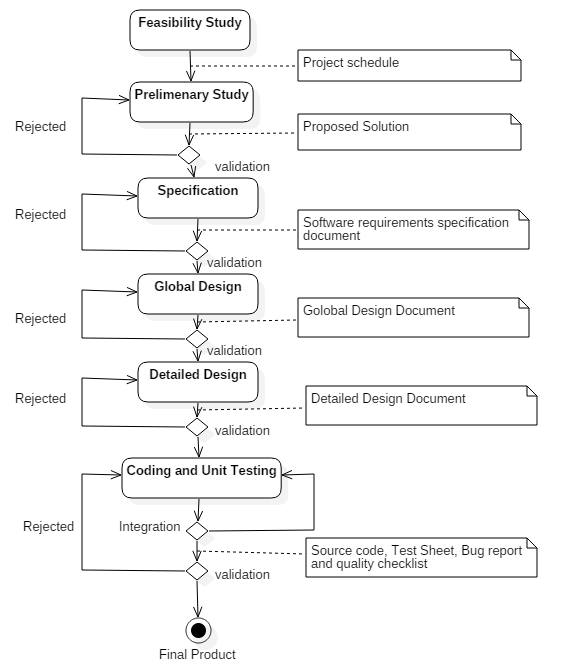
\includegraphics[width=14.8cm,height=17.8cm]{chapter1/fig2.png}
\end{center}
%légende de l'image
\caption{Integration Objects Work Methodology}
\label{fig2}
\end{figure}
\begin{itemize}
\item \textbf{Feasibility Study:} It is the first stage of the ISO process through which determines and to documents the project’s viability. \\ \textbf{Stage Output:} Project Schedule.
\item \textbf{Preliminary Study:} It represents an initial exploration of existing and possible solutions to the issue addressed. \\ \textbf{Stage Output:} Proposed solution.
\item \textbf{Specification:} This stage describes the client’s needs and determines the system features.\\ \textbf{Stage Output:} Software requirements specification document.
\item \textbf{Global Design:} The fourth stage describes the architecture of the product and its main parts. \\ \textbf{Stage Output:} Global design document.
\item \textbf{Detailed Design:} In this stage, we determine how to efficiently structure the main parts defined in the previous stage. \\\textbf{Stage Output:} Detailed design document.
\item \textbf{Coding and unit testing:} Developers have to implement the entire solution according to the design and to validate functional features. \\\textbf{Stage Output:} Source code, Test sheet, Bug report and quality checklist.
\end{itemize}
\section{Project Description}
\subsection{Scope}

This document is the \textbf{Graduation Project Dissertation} for a design and implementation of a \textbf{Big Data Management for Manufacturing Intelligence Application}. Throughout this document we will define the project's context and present it. This document will describe the methodology followed while realizing this project.


This project is a requirement for the final year in the \textbf{National School of Computer Science} in order to obtain the National Diploma of a Computer Sciences Engineer. It has been achieved during an internship
at \textbf{Integration Objects} that lasted 4 months starting from February $1^{st}$, 2017 to May $31^{th}$, 2017.

\subsection{Project Description}

\textbf{KnowledgeNet Analytics} is an out of the box data analysis software product, designed to meet operations needs in terms of knowledge mining in order to unlock hidden knowledge and profits within plant historical data. \textbf{KnowledgeNet Analytics} helps analyzing and investigating the plant process behavior and states, identifying opportunities to increase operational efficiency and reliability, and predicting abnormal conditions. One of the known issues in this field is how to manage huge volumes of data in term of storage, algorithms optimizations and presentation. The purpose of this project is to study and provide the best way for big data management.\\

The main objective of this project is to:
\begin{itemize}
\item Perform a literature review to understand the project scope
\item Engineer the best technical solution to load and manage huge volumes of data into a new built platform
\item Apply standard operations such as matrix operations and complex algorithms (PCA (Principal Components Analysis) and Linear Regression, etc.) using the best solution for big data
\item Compare results with other products
\end{itemize}
\section*{Conclusion}
This chapter was meant to set the general context in which our project took place. We presented the hosting company, isolated our project's goals and briefly described it. In the next chapter, we will establish a theoretical study, and we will be dealing with basic concepts relevant to our project while evaluating existing solutions.